\documentclass[17pt]{beamer}
\usetheme{Madrid}
\usepackage[utf8]{inputenc}
\usepackage[czech]{babel}
\usepackage[T1]{fontenc}
\usepackage{amsmath}
\usepackage{amsfonts}
\usepackage{amssymb}
\usepackage{graphicx}
\usepackage{multirow}
\usepackage{chngcntr}
\author{David Žáček}
\title[Volby do PSP ČR]{\small Analýza systému voleb do Poslanecké sněmovny České republiky}
%\setbeamercovered{transparent} 
\usepackage{array}
\newcolumntype{L}[1]{>{\raggedright\let\newline\\\arraybackslash\hspace{0pt}}m{#1}}
\newcolumntype{C}[1]{>{\centering\let\newline\\\arraybackslash\hspace{0pt}}m{#1}}
\newcolumntype{R}[1]{>{\raggedleft\let\newline\\\arraybackslash\hspace{0pt}}m{#1}}
\setbeamertemplate{navigation symbols}{} 
\institute{8.M} 
\date{7. března 2017} 
%\subject{} 
\begin{document}

\begin{frame}
\titlepage
\end{frame}

%\begin{frame}
%\tableofcontents
%\end{frame}

\begin{frame}{Úvod}
\center
\begin{block}{Poměrný volební systém}
Způsob voleb, kdy jsou mandáty rozdělovány ne podle pořadí subjektů ve volbách, ale dle poměrů hlasů které obdrželi.
\end{block}
\begin{block}{Úloha}
Rozdělte $N$ mandátů mezi strany účastnící se voleb tak, aby poměry zisku mandátů co nejlépe odpovídaly poměrům získu hlasů.
\end{block}
\begin{center}
%\begin{tabular}{|c|c|c|c|c|c|c|}
%\hline
%Hlasy & 4700 & 1600 & 1590 & 1200 & 600 & 310  \\ \hline
%\end{tabular}
\end{center}
\end{frame}

%\begin{frame}{Úvod}
%\center
%Pro $N=10$:
%\bigskip
%\begin{center}
%\begin{tabular}{|c|c|c|c|c|c|c|}
%\hline
%Hlasy & 4700 & 1600 & 1590 & 1200 & 600 & 310  \\ \hline
%Podíl & 4.7  & 1.6  & 1.59 & 1.2  & 0.6 & 0.31 \\ \hline
%      & 5    & 2    & 2    & 1    & 0   & 0    \\ \hline
%      & 5    & 2    & 1    & 1    & 1   & 0    \\ \hline
%      & 4    & 2    & 2    & 1    & 1   & 0    \\ \hline
%\end{tabular}
%\end{center}
%\end{frame}

\begin{frame}{Počátky poměrných systémů}
\begin{center}

\includegraphics[scale=0.2]{zdroje/const.jpg}
\end{center}
\end{frame}

%\begin{frame}{Bez určeného počtu}
%\begin{itemize}
%\item Předem zvolená kvóta: $K$
%\item Počet hlasu pro stranu: $H_{x}$
%\item Zisk mandátů: $\left\lfloor\frac{H_{x}}{K}\right\rfloor$
%\end{itemize}
%\end{frame}

\begin{frame}{Metoda nejvyšších zbytků}
\begin{itemize}
\item Počet rozdělovaných mandátů $N$
\item Kvóta: $K=\frac{H_{c}}{N}$
\item Zisk mandátů: $\left\lfloor\frac{H_{x}}{K}\right\rfloor+\{0;1\}$
\end{itemize}
\end{frame}

\begin{frame}{Ovlivnění třetí stranou}
\begin{center}
\begin{tabular}{|c|c|c|c|}
\hline 
 & Hlasy & Ku kvótě & Mandáty \\ 
\hline 
A & 8955 & 8955/100=89.55 & 90 \\ 
\hline 
B & 1045 & 1045/100=10.45 & 10 \\ 
\hline 
C & 500 & 500/100=5 & 5 \\ 
\hline 
\end{tabular} 
\end{center} 
\begin{center}
\begin{tabular}{|c|c|c|c|}
\hline 
 & Hlasy & Ku kvótě & Mandáty \\ 
\hline 
A & 8955 & 8955/100.14=89.42 & 89 \\ 
\hline 
B & 1045 & 1045/100.14=10.44 & 11 \\ 
\hline 
C & 515 & 515/100.14=5.14 & 5 \\ 
\hline 
\end{tabular} 
\end{center}
\end{frame}

\begin{frame}{Alabamský paradox}
\begin{center}
\begin{tabular}{|c|c|c|c|c|c|}
\hline 
 &  & \multicolumn{2}{c|}{10 mandátů} & \multicolumn{2}{c|}{11 mandátů} \\ 
\hline 
 & Hlasy & Ku kvótě & Zisk & Ku kvótě & Zisk \\ 
\hline 
A & 300 & 4,286 & 4 & 4,714 & 5 \\ 
\hline 
B & 300 & 4,286 & 4 & 4,714 & 5 \\ 
\hline 
C & 100 & 1,426 & 2 & 1.571 & 1 \\ 
\hline
\end{tabular} 
\end{center}
\end{frame}

\begin{frame}{Metody nejvyšších průměrů}
\begin{itemize}
\item Počet rozdělovaných mandátů $N$
\item Zisk mandátů: $\left\langle\frac{H_{x}}{K}\right\rangle$
\item $\langle$\hspace{0.15cm}$\rangle$ je zaokrouhlení.
\item $K$ je určeno tak, aby bylo rozděleno \\ právě $N$ mandátů.
\end{itemize}
\end{frame}

%\begin{frame}{Metody nejvyšších průměrů}
%\begin{itemize}
%\item D'Hondtova metoda $\left\lfloor\frac{H_{x}}{K}\right\rfloor$
%\item Metoda Sainte-Lague $\left[\frac{H_{x}}{K}\right]$
%\item Adamsova metoda $\left\lceil\frac{H_{x}}{K}\right\rceil$
%%\item Metoda Huntington-Hill: zaokrouhlení dle geometrického průměru.
%\end{itemize}
%\end{frame}

\begin{frame}{Metody nejvyšších průměrů}
\begin{itemize}
\item Běžně se výpočet dle této metody provdí pomocí řady \uv{mezí zaokrouhlení}
\item Pro zaokrouhlení dolu (D'Hondt): řada $1; 2; 3; 4; ...$
\item Pro zaokrouhlení běžné (Sainte-Lague): řada $0{,}5; 1{,}5; 2{,}5; 3{,}5; ...$
\end{itemize}
\end{frame}

\begin{frame}{Řada mezí zaokrouhlení}
\begin{itemize}
\item A:44 B:40 C:16
\item Pro 6 mandátů:
\end{itemize}
\begin{center}
\begin{tabular}{|C{2cm}|C{2cm}|C{2cm}|C{2cm}|}
\hline 
 & A & B & C \\ 
\hline 
1 & \emph{\textbf{44}} & \emph{\textbf{40}} & \emph{\textbf{16}} \\ 
\hline 
2 & \emph{\textbf{22}} & \emph{\textbf{20}} & 8 \\ 
\hline 
3 & \emph{\textbf{14,67}} & 13,33 & 5,33 \\ 
\hline 
4 & 11 & 10 & 4 \\ 
\hline 
\end{tabular} 
\end{center}
\end{frame}

\begin{frame}{Hypotetické volby}
\begin{itemize}
\item 200 poslanců
\item Tři strany A, B, C
\item A:49\% B:45\% C:6\%
\item Homogenně rozložená podpora
\end{itemize}
\end{frame}

\begin{frame}{Výsledky}
\begin{center}
\begin{tabular}{|c|c|c|c|} \hline
  & A & B & C \\ \hline 
Přesný poměr & 98 & 90 & 12\\ \hline
\end{tabular}
\end{center} 
\end{frame}

\begin{frame}{Výsledky}
\begin{center}
\begin{tabular}{|c|c|c|c|} \hline
  & A & B & C \\ \hline 
Přesný poměr & 98 & 90 & 12\\ \hline
SR & 98 & 90 & 12\\ \hline
\end{tabular}
\end{center} 
\end{frame}

\begin{frame}{Výsledky}
\begin{center}
\begin{tabular}{|c|c|c|c|} \hline
  & A & B & C \\ \hline 
Přesný poměr & 98 & 90 & 12\\ \hline
SR & 98 & 90 & 12\\ \hline
ČR & 102 & 94 & 3\\ \hline
\end{tabular}
\end{center} 
\end{frame}

\begin{frame}{Výsledky}
\begin{center}
\begin{tabular}{|c|c|c|c|} \hline
  & A & B & C \\ \hline 
Přesný poměr & 98 & 90 & 12\\ \hline
SR & 98 & 90 & 12\\ \hline
ČR & 102 & 94 & 3\\ \hline
UK/USA & 200 & 0 & 0\\ \hline
\end{tabular}
\end{center} 
\end{frame}

\begin{frame}{Výsledky}
\begin{center}
\begin{tabular}{|c|c|c|c|} \hline
  & A & B & C \\ \hline 
Přesný poměr & 98 & 90 & 12\\ \hline
SR & 98 & 90 & 12\\ \hline
ČR & 102 & 94 & 3\\ \hline
UK/USA & 200 & 0 & 0\\ \hline
\end{tabular}
\end{center} 
V roce 2006 opravdu získala Strana zelených $6{,}29\%$ hlasu ale jen $3\%$ poslanců. 
\textbf{Jak je to možné?}
\end{frame}

\begin{frame}{Kraje}
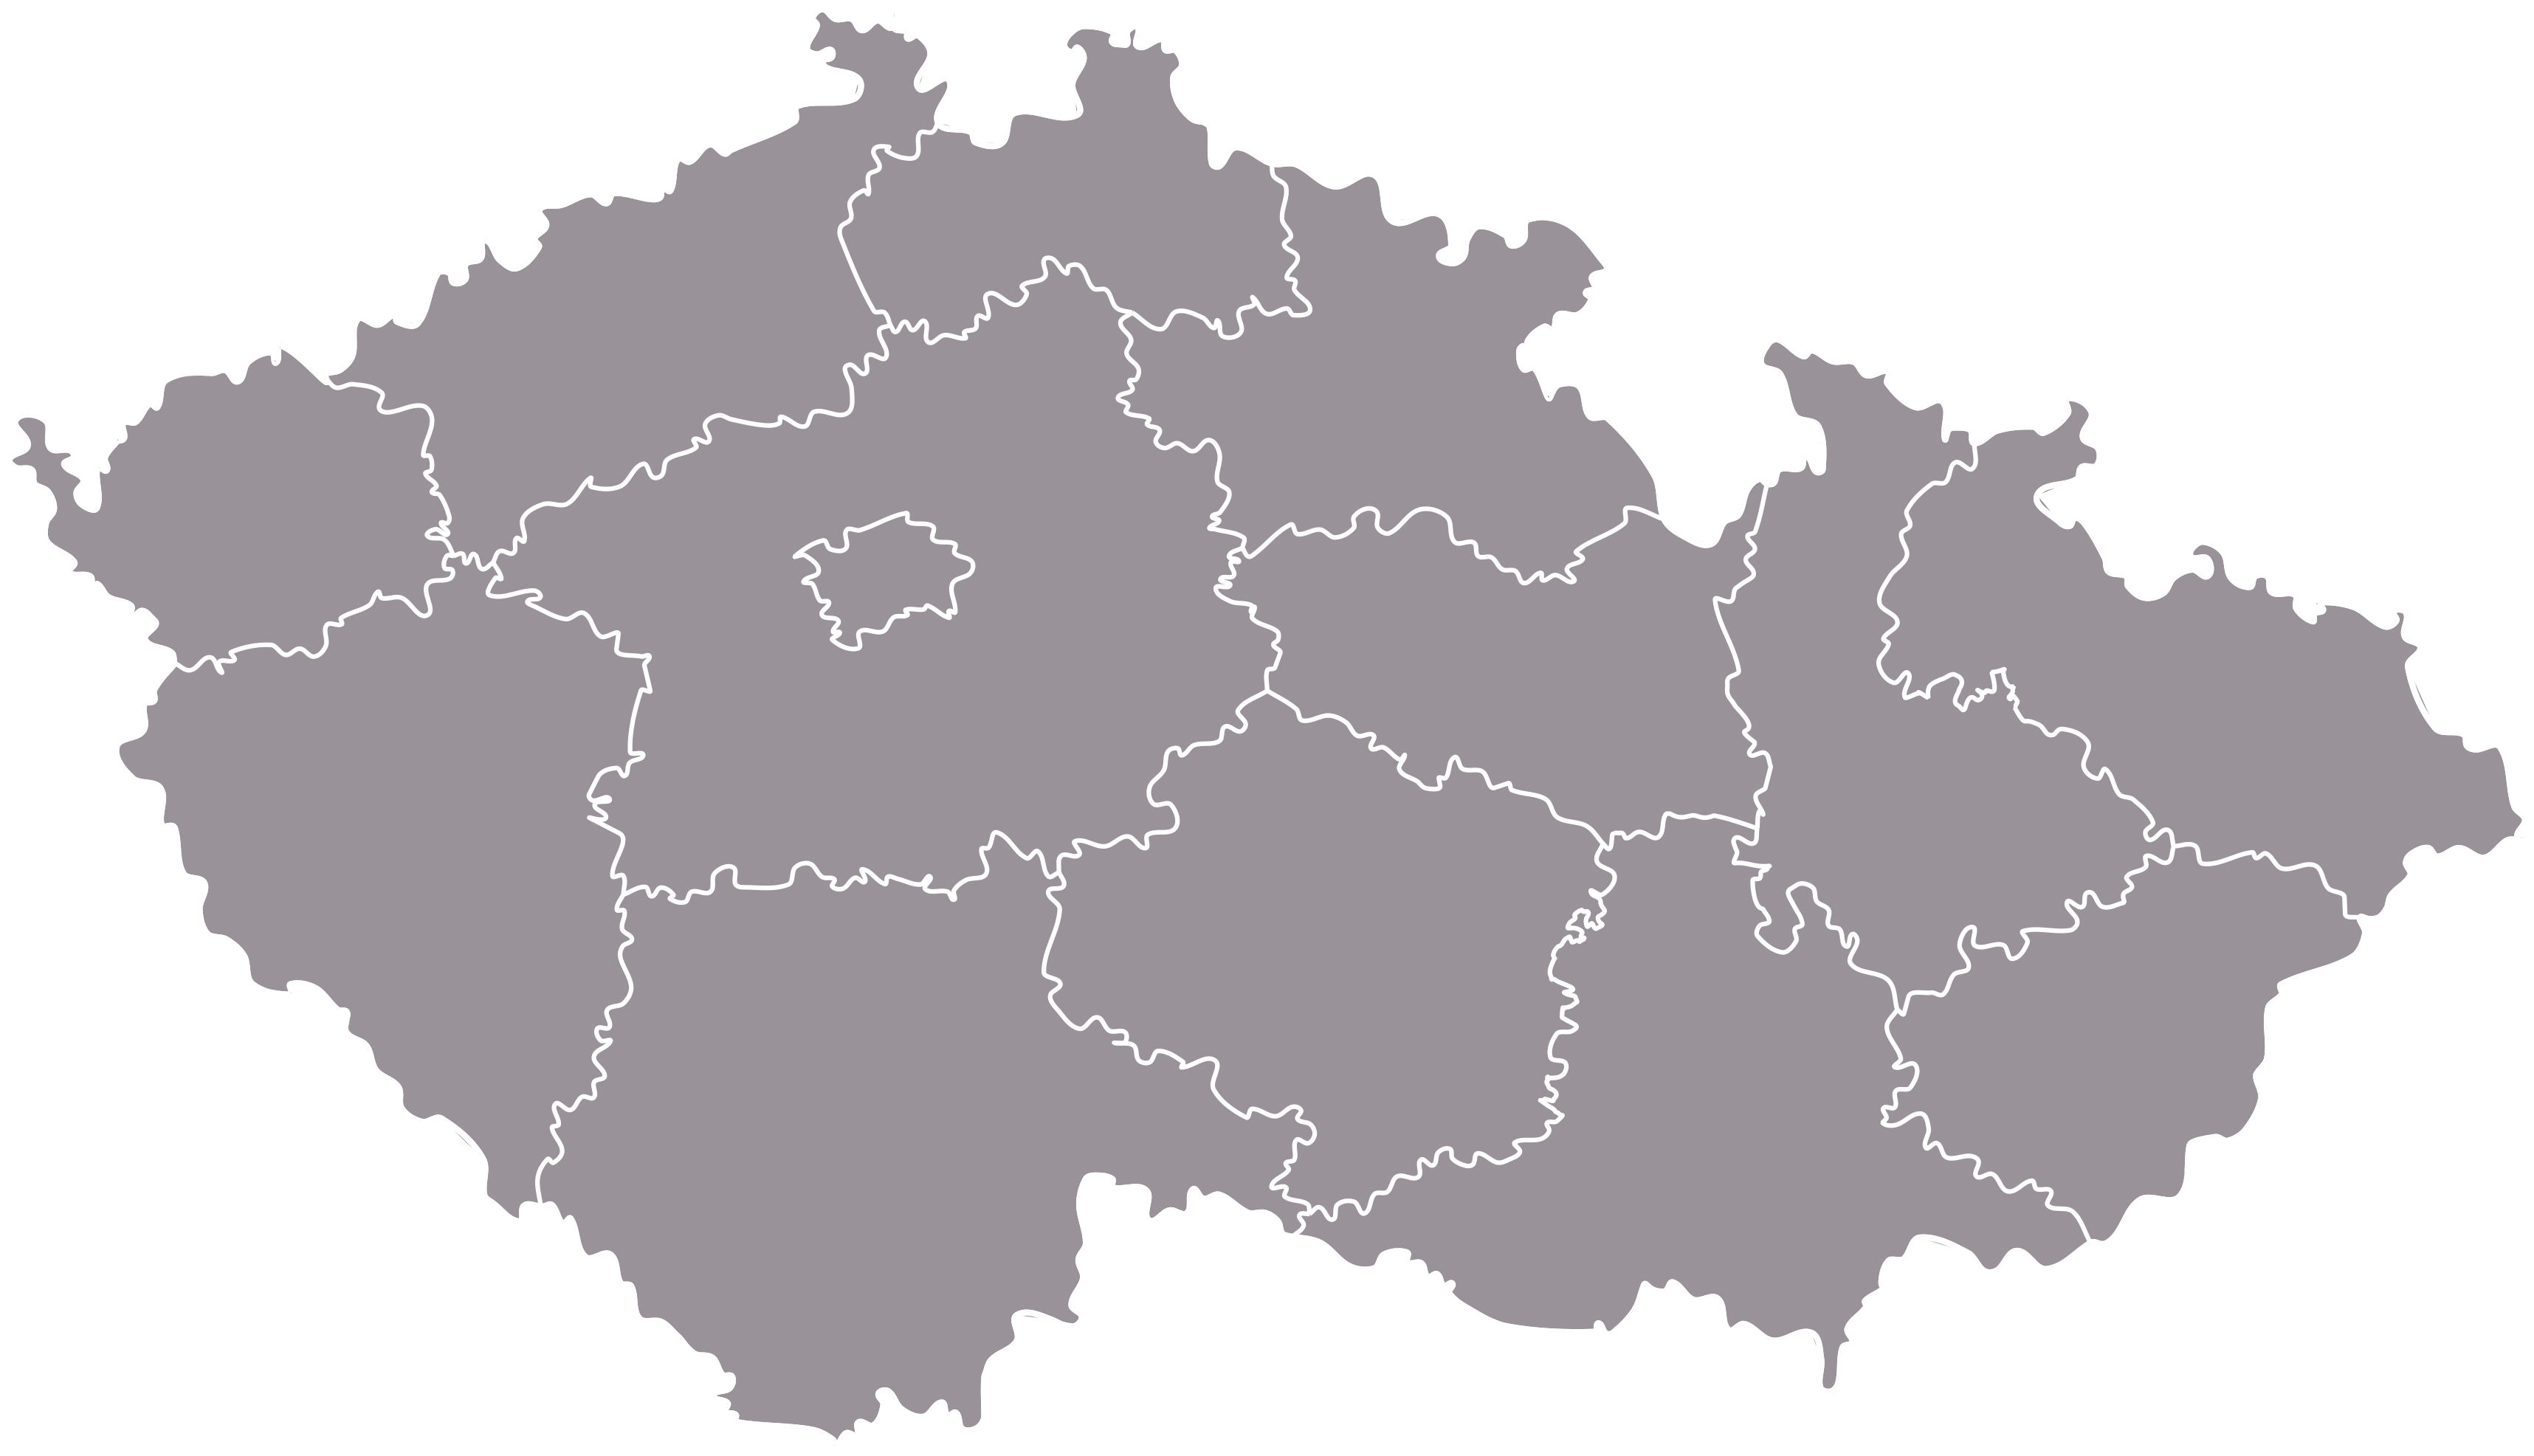
\includegraphics[scale=0.1]{zdroje/kraje.png}
\end{frame}

\begin{frame}{ČR (200) 2006}
\footnotesize
\begin{tabular}{|c|c|c|c|c|c|c|} \hline
 & \multicolumn{2}{c|}{Výsledky} & Přesně & D'Hondt & Adams & Kvóta\\
\hline ODS & 1892475 & 81 & 75.25 & 76 & 75 & 75\\
\hline ČSSD & 1728827 & 74 & 68.74 & 69 & 68 & 69\\
\hline SZ & 336487 & 6 & 13.38 & 13 & 14 & 14 \\
\hline KSČM & 685328 & 26 & 27.25 & 27 & 27 & 27 \\
\hline KDU-ČSL & 386706 & 13 & 15.38 & 15 & 16 & 15 \\
\hline
\end{tabular}
\end{frame}

\begin{frame}{Karlovarský kraj (5) 2006 a 2013}
\begin{center}
\begin{tabular}{|c|c|c|}
\hline
Strana  & \multicolumn{2}{c|}{Zisk}   \\ \hline
ODS     & 38,33\% & 2 \\ \hline
ČSSD    & 34,98\% & 2 \\ \hline
SZ      & 7,17\% & 0 \\ \hline
KSČM    & 15,84\% & 1 \\ \hline
KDUČSL & 3,68\% & 0  \\ \hline
\end{tabular}
\begin{tabular}{|c|c|c|}
\hline
Strana  & \multicolumn{2}{c|}{Zisk}     \\ \hline
ČSSD    & 24,28\% & 2 \\ \hline
TOP09   & 11,47\% & 0 \\ \hline
ODS     & 7,65\% & 0  \\ \hline
KDUČSL & 3,82\% & 0 \\ \hline
Úsvit   & 9,48\% & 0 \\ \hline
ANO2011 & 24,25\% & 2 \\ \hline
KSČM    & 19,02\% & 1 \\ \hline
\end{tabular}
\end{center}
\end{frame}

\begin{frame}{Kraje -- řešení}
\footnotesize
\begin{tabular}{|c|c|c|c|c|c|c|} \hline
 & \multicolumn{2}{c|}{Výsledky} & Přesně & D'Hondt & Adams & Kvóta\\
\hline ODS & 1892475 & 81 & 75.25 & 76 & 75 & 75\\
\hline ČSSD & 1728827 & 74 & 68.74 & 69 & 68 & 69\\
\hline SZ & 336487 & 6 & 13.38 & 13 & 14 & 14 \\
\hline KSČM & 685328 & 26 & 27.25 & 27 & 27 & 27 \\
\hline KDU-ČSL & 386706 & 13 & 15.38 & 15 & 16 & 15 \\
\hline
\end{tabular}
\end{frame}

\begin{frame}{Závěr}
\begin{itemize}
\item Existuje mnoho způsobů jak dělt mandáty mezi strany.
\item Každý má své pro i proti.
\item Volební systém pro zkoumané volby není ideální.
\item Existují způsoby jak ho učinit férovějším.
\item Způsoby rozdělování lze uplatnit i jinde.
\end{itemize}
\end{frame}

\end{document}
